\documentclass[aps,prapplied,longbibliography]{article}
\usepackage{physics}
\usepackage{amssymb}
\usepackage{amsmath}
\usepackage{qcircuit}

\usepackage{geometry}
\geometry{
  margin=2cm  
}

\usepackage{xcolor}
\usepackage{graphicx}
\usepackage{float}
\usepackage{cite}
\usepackage{listings}
\lstset{
  basicstyle=\ttfamily,
  mathescape,
  emph={for, do, end},
  emphstyle={\color{blue}\bf}
}

\usepackage{caption}
\usepackage{subcaption}

% Change color of citation links
\usepackage[colorlinks=true,linkcolor=blue,citecolor=blue]{hyperref}

\title{QOSF Mentorship Program: Task 1}
\author{Leander Reascos}

\begin{document}
    \maketitle

    \begin{abstract}
        This work introduces a quantum algorithm aimed at verifying Goldbach's conjecture, a famous mathematical hypothesis asserting that any even integer greater than two can be expressed as the sum of two prime numbers. Leveraging quantum parallelism and the Grover's algorithm, our proposed quantum circuit efficiently searches for pairs of prime numbers that satisfy this conjecture. Through comprehensive analysis and simulations, we demonstrate that the quantum approach exhibits a superior asymptotic complexity of $\mathcal{O}(N)$ compared to the classical approach's $\mathcal{O}(N^2)$, making it increasingly efficient as problem size grows. Our results confirm the practical viability of the proposed quantum circuit and underscore the potential of quantum computing in tackling complex mathematical challenges.
    \end{abstract}

    \section{Introduction}

    This report aims to illustrate the solution to Task 1 of the Screening task for the QOSF Mentorship Program. Task 1 requires finding two prime numbers from a given list that sum up to a positive integer. Firstly, it is clear that the task involves developing a quantum algorithm to verify Goldbach's conjecture. In simple terms, Goldbach's conjecture states that any even integer greater than two can be expressed as the sum of two prime numbers \cite{wang2002goldbach}. While this conjecture remains unsolved, significant efforts have been made to prove it. Consequently, various classical algorithms have been developed to test this conjecture with very large numbers such as $4\cdot10^{14}$ \cite{richstein2001verifying}.

    Therefore, quantum computers could play a significant role in verifying this conjecture. This can be achieved by harnessing quantum parallelism, which enables operations to be applied to a superposition of states. This approach reduces the computational workload, as illustrated by the Deutsch-Jozsa algorithm, which serves as a compelling example of this concept \cite{collins1998deutsch}. The Deutsch-Jozsa algorithm efficiently verifies a function by determining whether it is constant or balanced, and it does so exponentially faster on a quantum computer compared to classical methods \cite{collins1998deutsch}.

    However, to extract meaningful information from these quantum operations, it is essential to devise a way to measure only the desired outcome accurately. In this context, Grover's algorithm \cite{grover1996fast} emerges as the preferred method to pursue, as it provides a technique to amplify the probability of measuring the desired outcome, making it a powerful tool for quantum computation tasks like verifying Goldbach's conjecture \cite{latorre2013quantum, prudencio2013goldbach}.


    \section{Classical approach}

    Since in this report we are only going to compare our quantum approach with the naive classical approach this section aims to explain what it is this classical method to evaluate the Golbach's conjecture. Thus, let's consider a number $n$ which we want to find the two prime numbers  $p$ and $q$ that added results in this number. These prime numbers $p$ and $q$ are contained in a list of $N$ prime numbers.

    \begin{equation}
        n = p + q,\hspace{1cm}p,q\in\text{Primes}
    \end{equation}

    Therefore, the naive classical approach consists of taking the list of $N$ numbers and computing all possible sums of two numbers, resulting in a search space of $N^2$. This can be illustrated in the table \ref{tab:SumsClassical}.

    \begin{table}[h]
        \centering
        \caption{Sum of all possible pairs of prime numbers $P_i$ and $P_j$ from a list of $N$ prime numbers.}
        \label{tab:SumsClassical}
        \begin{tabular}{c|cccc}
            & $P_1$ & $P_2$ & $P_3$ & $\ldots$ \\
            \hline
        $P_1$ & $P_1 + P_1$ & $P_1 + P_2$ & $P_1 + P_3$ & $\ldots$ \\
        $P_2$ & $P_2 + P_1$ & $P_2 + P_2$ & $P_2 + P_3$ & $\ldots$ \\
        $P_3$ & $P_3 + P_1$ & $P_3 + P_2$ & $P_3 + P_3$ & $\ldots$ \\
        $\vdots$ & $\vdots$ & $\vdots$ & $\vdots$ & $\ddots$ \\
        \end{tabular}
    \end{table}

    It is possible to reduce the search space to $\frac{N^{2}}{2}$ due to the commutative property of addition. Therefore, in the worst case, it is required to compute $\frac{N^{2}}{2}$ sums and search in $\frac{N^2}{2}$ elements. We can denote this complexity as $\mathcal{O}_{a}(N^2)$ for the growth in the number of sums and $\mathcal{O}_s(N^2)$ for the growth in the number of searches, respectively.

    \section{Quantum Approach}

    \subsection{Quantum Adder}

    The quantum approach that we have decided to implement follows the same idea as the classical approach. Since quantum computers encode information in qubits, which are the quantum analog of classical bits, the addition of two integers should be carried out by implementing the addition of two binary numbers.

    Classically, adding two binary integers is achieved through the use of just two fundamental logical gates: the $AND$ gate ($\cdot$) and the $XOR$ gate ($\oplus$). The $XOR$ gate computes the bit-by-bit sum (see Table \ref{tab:XOR}), while the $AND$ gate determines if a carry bit is needed in the addition process.

    \begin{table}[h]
        \centering
        \caption{$XOR$ Truth Table}
        \label{tab:XOR}
        \begin{tabular}{cc|c}
            A & B & A $\oplus$ B \\
            \hline
            0 & 0 & 0 \\
            0 & 1 & 1 \\
            1 & 0 & 1 \\
            1 & 1 & 0 \\
            \hline
        \end{tabular}
    \end{table}

    For example, to add the integers 3 and 2, we first need to represent them in binary format as $11_2$ and $10_2$, respectively. The binary addition of these two integers is as follows:

    \begin{equation}
        \begin{array}{c@{}c@{}c@{}c@{\hspace{0.5em}}r}
            &   & 1 & 1 & {\text{(Carry)}} \\
            &   & 1 & 1 & \text{(3 in binary)} \\
          + &   & 1 & 0 & \text{(2 in binary)} \\
          \hline
            & 1 & 0 & 1 & \text{(5 in binary)}
        \end{array}
    \end{equation}

    Hence, if we want to follow the classical approach, it is required to implement a quantum operator $U^+$ that acts on three quantum registers, each containing $m$ qubits. The first $A$ and second registers $B$ encode the first and second summands $a$ and $b$ in binary, respectively, while the last one serves as an ancillary register used to carry $\ket{carry}$ information for the sum. Thus, the result of the sum would be encoded in the $B$ register and the most significant quantum bit of the carry register.

    \begin{equation}
        U^+\ket{a}_m\ket{b}_m\ket{Carry}_m = \ket{a}_m\ket{a+ b}_{m+1}\ket{Carry}_{m-1}
    \end{equation}

    The subscript $l$ in each state $\ket{\alpha}_l$ indicates that this register encodes the integer $\alpha$ with $l$ qubits. Additionally, if we encode the registers $A$ and $B$ in equal superpositions of $N$ numbers each, it becomes possible to perform all the possible $N^2$ sums using only one application of the addition operator $U^+$, which we are going to refer to as the Quantum Adder. The quantum circuit that implements this Quantum Adder operator $U^+$ can be observed in Figure \ref{fig:QuantumAdder}.

    \begin{figure}
        \centering
        \scalebox{1}{
        \Qcircuit @C=1.7em @R=1em {
            \lstick{} & \ctrl{3} & \ctrl{3} \barrier{8} & \qw & \qw &\qw & \qw & \qw \barrier{8} & \qw  \hspace{1cm} \dots \\
            \lstick{} & \qw & \qw & \qw & \ctrl{3} & \ctrl{3} & \qw & \qw & \qw  \hspace{1cm} \dots \\
            \lstick{} & \hspace{-0.5cm}\vdots & {~} & {~} & {~} & {~} & {~} & {~}  & {~} 
            \inputgroupv{1}{3}{.8em}{.8em}{\ket{a}} \\
            \lstick{} & \ctrl{3} & \targ & \qw & \qw & \qw & \qw & \qw & \qw\\
            \lstick{} & \qw & \qw & \qw & \ctrl{3} & \targ & \ctrl{2} & \targ & \qw  \hspace{1cm} \dots \\
            \lstick{} & \hspace{-0.5cm}\vdots & {~} & {~} & {~} & {~} & {~} & {~} & {~} 
            \inputgroupv{4}{6}{.8em}{.8em}{\ket{b}} \\
            \lstick{} & \targ & \qw & \qw & \qw & \qw & \ctrl{1} & \ctrl{-2} & \qw \hspace{1cm} \dots \\
            \lstick{} & \qw & \qw & \qw & \targ & \qw & \targ & \qw & \qw \hspace{1cm} \dots \\
            \lstick{} & \hspace{-0.5cm}\vdots & {~} & {~} & {~} & {~} & {~} & {~} & {~} 
            \inputgroupv{7}{9}{.8em}{.8em}{\ket{Carry}\hspace{0.8cm}}\\
        }}
        \caption{he figure represents the Quantum Adder operator $U^+$. The algorithm adds two registers $A$ and $B$ encoding the integers $a$ and $b$ in their quantum binary representations $\ket{a}$ and $\ket{b}$. The carry state starts as $\ket{Carry}\equiv\ket{00\dots0}$. The algorithm operates similarly to its classical counterpart. First, the quantum version of the $AND$ gate, which is a Toffoli gate, is applied. Then, the $CNOT$ gate, serving as the quantum $XOR$ gate, adds the quantum bits. Both of these operations are shown in the first stage delimited by the barrier. The subsequent steps involve applying the Toffoli gate using the quantum bit and the carry qubit, which holds the carry from the previous operation. This is followed by another $CNOT$ operation to sum the carry qubit. This process is applied to all the qubits.}  
        \label{fig:QuantumAdder}
    \end{figure}
    
    Let's consider two lists of integers, denoted as $X$ and $Y$. The register $A$ encodes, in a uniform superposition, all the integers in list $X$ using $m$ qubits, while the register $B$ encodes the integers from list $Y$ in a similar manner with the same number of qubits.

    \begin{equation}
        \begin{aligned}
            U^+ \frac 1N\sum_{\substack {x\in X,\\y\in Y}} \ket{x}_m  \ket{y}_m  \ket{Carry}_m &= \frac 1N \sum_{\substack {x\in X,\\y\in Y}} U^+ \ket{x}_m\ket{y}_m\ket{Carry}_m\\
            &= \frac 1N \sum_{\substack {x\in X,\\y\in Y}} \ket{x}_m\ket{x+y}_{m+1}\ket{Carry}_{m-1}
        \end{aligned}
    \end{equation}

    Therefore, it is evident that after the application of the Quantum Adder operator $U^+$ over a uniform superposition of $N$ integers encoded in each register, it is possible to compute all the possible sums of two integers $x\in X$ and $y \in Y$. Thus, if the list of integers $X$ and $Y$ corresponds to the list of $N$ prime numbers, by preparing both registers $A$ and $B$ in an equal superposition, it is possible to compute the sums of all $N^2$ pairs of these $N$ prime numbers.

    \subsection{Grover's Algorithm}

    However, having all the possible results doesn't solve the problem, as when the registers are measured, the information collapses with equal probability for each sum. To address this challenge, we employ Grover's algorithm. This quantum algorithm is designed to search for a specific element or elements in an unindexed database and has a complexity on the order of $\mathcal{O}_s(\sqrt{N})$, where $N$ represents the number of elements in the dataset \cite{grover1996fast}.

    Therefore, by utilizing Grover's algorithm, we can enhance the probability of measuring the state that encodes the result. In simpler terms, we aim to measure the state $\ket{p}\ket{p+q}$ such that $n = p+q$, where $n$ is our target integer to be expressed in terms of two prime numbers, $p$ and $q$.

    The Grover's algorithm used in this project is its generalized version since the search space is not a uniform superposition over all possible states encoded by the qubits. Instead, the search space is a uniform superposition over all possible sums of two prime integers contained in a given list. Thus, the generalized Grover iterator operator $G$ for this particular problem can be seen below \cite{brassard1998quantum}.

    \begin{equation}
        G = U^+ S_0 (U^+)^{\dagger} S_{n}
    \end{equation}

    Here, the oracle is represented by $S_n$, which consists of an operator that marks the state encoding the desired target number $n$ with $-1$. $S_0$ marks the state zero with $-1$, as is typically done in Grover's algorithm. To implement the oracle $S_n$, a controlled Pauli-$Z$ gate is applied to the most significant qubit where the sum is encoded. Since we need to mark the desired binary representation of the number $n$ with $-1$, the remaining bits determine the control state for this respective qubit. If the most significant bit of $n$ is zero, a Pauli-$X$ gate is applied before and after the controlled Pauli-$Z$ gate. For example, if $n=6$ ($\ket{0110}$), the circuit $S_6$ is illustrated in Figure \ref{fig:Oracle}.

    \begin{figure}[h]
        \centering
        \scalebox{1}{
        \Qcircuit @C=1.7em @R=1em {
            \lstick{} & \qw & \ctrlo{3} & \qw & \qw \\
            \lstick{} & \qw & \ctrl{2} & \qw & \qw \\
            \lstick{} & \qw & \ctrl{1} & \qw & \qw 
            \inputgroupv{1}{3}{.8em}{.8em}{\ket{b}}\\
            \lstick{\ket{Carry}_{msb}} & \gate{X} & \gate{Z} & \gate{X} & \qw 
        }}
        \caption{The figure represents the oracle $S_6$ for the number $n=6$. The oracle marks the state $\ket{0110}$ with $-1$. Please note that the most significant bit (MSB) of the binary representation of $n$ is encoded in the MSB of the carry register.}
        \label{fig:Oracle}
    \end{figure}

    Consequently, by applying the Grover iterators a sufficient number of times, it becomes possible to amplify the probability of measuring the state $\ket{p}\ket{p+q}$ such that $n=p+q$. Thus, it is straightforward to obtain $q = n-p$ and solve the problem. Furthermore, the exact number of times that the Grover iterator $G$ needs to be applied is unknown, as we do not know the answer or the number of solutions in advance. Therefore, we will increase the number of iterations if necessary.

    In essence, our solution is reached by executing the quantum circuit $N_{\text{shoots}}$ times, starting with one Grover iteration. After each run, we check the outcomes to see if our solution has been found. If it hasn't been found, the number of iterations of $G$ is increased by one. However, due to limitations in classical resources for simulation or, in the case of real devices, the presence of decoherence, we impose a maximum value $max_{\text{iterations}}$ for the number of iterations of $G$. When this maximum value is reached, the number of $G$ iterations is reset to one. Additionally, since each execution of this algorithm and the subsequent classical processing represent an attempt to find the solution, we also limit the number of attempts to $max_tries$. This is because there are cases where $n$ cannot be expressed in terms of the prime numbers provided in the list. The final quantum circuit with one Grover iteration can be observed in Figure \ref{fig:QCG}.

    \begin{figure}[h]
        \centering
        \scalebox{1}{
            \Qcircuit @C=1.7em @R=1em {
                \lstick{\ket{a}} & {/^m} \qw & \multigate{2}{U^+} & \qw & \multigate{2}{\left(U^+\right)^\dagger} & \qw &\multigate{2}{U^+} & \qw \\
                \lstick{\ket{b}} & {/^m} \qw & \ghost{U^+} & \multigate{1}{S_n} & \ghost{\left(U^+\right)^\dagger} & \multigate{1}{S_0} & \ghost{U^+} & \qw \\
                \lstick{\ket{Carry}} & {/^m} \qw & \ghost{U^+} & \ghost{S_n} & \ghost{\left(U^+\right)^\dagger} & \ghost{S_0} & \ghost{U^+} & \qw
                \gategroup{1}{4}{3}{7}{.7em}{--}
        }}
        \caption{The figure shows the final quantum circuit to test Goldbach's conjecture. The dashed box represents one Grover iteration.}
        \label{fig:QCG}
    \end{figure}

    One possible solution to overcome the challenge of determining the ideal number of Grover's iterations is to employ the Quantum Counting algorithm, which applies the Quantum Phase Estimation (QPE) algorithm to the Grover iterator $G$ \cite{brassard1998quantum}. However, due to the additional executions and the increased quantum resources required to implement this approach, we have chosen to use the iterative search method as described previously. Nevertheless, the option of using Quantum Counting remains a viable possibility.

    \section{Results}

    This section aims to test the proposed quantum circuit and compare the complexity of our quantum solution with the classical one. To facilitate this comparison, we will present an analysis of the theoretical asymptotic complexity of both the quantum and the naive classical approaches. Subsequently, we will simulate the results for a range of even values of $n$ within the interval $[2,100]$. It's important to note that we only consider even numbers in this analysis since Goldbach's conjecture, as presented in this text, is supposed to hold only for even integers.

    \subsection{Theoretical Complexity}

    Let's recap the classical complexity as previously discussed. To verify Goldbach's conjecture for a specific even integer $n$ using a list of $N$ prime numbers, the classical naive algorithm has an asymptotic complexity of $\mathcal{O}_a(N^2)$ for both the number of sums and the number of searches. Furthermore, if there are $k\geq 1$ solutions in the search space of $\frac{N^2}{2}$, in the worst case, it would be required to perform $\frac{N^2}{2}- k$ additional searches, which still maintains an asymptotic complexity of $\mathcal{O}_a(N^2)$ for both summing and searching.
    
    The quantum approach presented in this text has an asymptotic complexity primarily limited by Grover's algorithm. For performing all the additions, it only requires one application of the Quantum Adder operator $U^+$. Therefore, considering the same example with a search space of $N^2$ and $2k$ solutions, thanks to the symmetry of the search space due to the commutative property of addition, the asymptotic complexity of Grover's algorithm is given by $\mathcal{O}\left(\frac{N}{\sqrt{2k}}\right)$. Since each Grover iteration involves two Quantum Adder operations and one search operation, the resulting asymptotic number of additions is $\frac{N}{\sqrt{2k}} + 1$ and $\frac{N}{\sqrt{2k}}$ searches.

    Given that our proposed algorithm runs the circuit $N_{\text{shoots}}$ times and performs $n_{\text{tries}}$ attempts, the final number of additions and searches can be calculated as follows.

    \begin{equation}
        N_{additions} = \sum_{n_{try}=1}^{n_\text{tries}} N_\text{shoots} \left(\frac{N}{\sqrt{2k}} + 1\right) = n_\text{tries} N_\text{shoots} \left(\frac{N}{\sqrt{2k}} + 1\right)
    \end{equation}

    \begin{equation}
        N_{searches} = \sum_{n_{try}=1}^{n_\text{tries}} N_\text{shoots} \frac{N}{\sqrt{2k}} = n_\text{tries} N_\text{shoots} \frac{N}{\sqrt{2k}}
    \end{equation}

    If we assume that the number of solutions is small in comparison to the search space $k\ll N^2$ and we also keep the number of shots and attempts small $N_\text{shoots}\ll N^2$ and $n_\text{tries}\ll N^2$, then the final asymptotic complexity of additions and searches can indeed be approximated as $\mathcal{O}_{a/s}(N)$. In this scenario, the quantum approach becomes efficient, and its complexity is linear with respect to the size of the search space, making it favorable for solving the problem efficiently.

    \subsection{Simulation Results}

    To effectively verify if the algorithm works and compare the actual complexity with the previous analysis, we conducted a simulation of the quantum circuit to find prime numbers $p$ and $q$ that, when added, yield $n$ for even integers $n$ in the range $[2, 100]$. This simulation involved a list of all prime numbers from $1$ to $n$ (not inclusive). The simulation parameters used were $N_\text{shoots}=5$, $max_\text{tries}=10$, and $max_\text{iterations}=5$. We counted the number of additions and searches performed. Additionally, it's worth noting that we also considered a classical search process required to verify the results of the $N_{\text{shoots}}$ simulation. The simulation described above was repeated 10 times to obtain statistical results regarding the complexity of the proposed quantum circuit. 

    Furthermore, the results were verified for all the integers $n$ under analysis, and the proposed quantum circuit successfully solved the problem for all of them. The number of additions and searches performed to obtain the result for a given array of $N$ prime numbers is depicted in Figure \ref{fig:Results}. In the figure, it is possible to see that for small-sized lists of primes, the classical approach remains better than our solution. However, as the size of the problem increases, the quantum solution proposed in this work outperforms the classical solution. It becomes evident that the complexity of the quantum algorithm scales as described in the previous quantum complexity analysis, at least within the statistical error considered in this study.

    \begin{figure}[H]
        \centering
        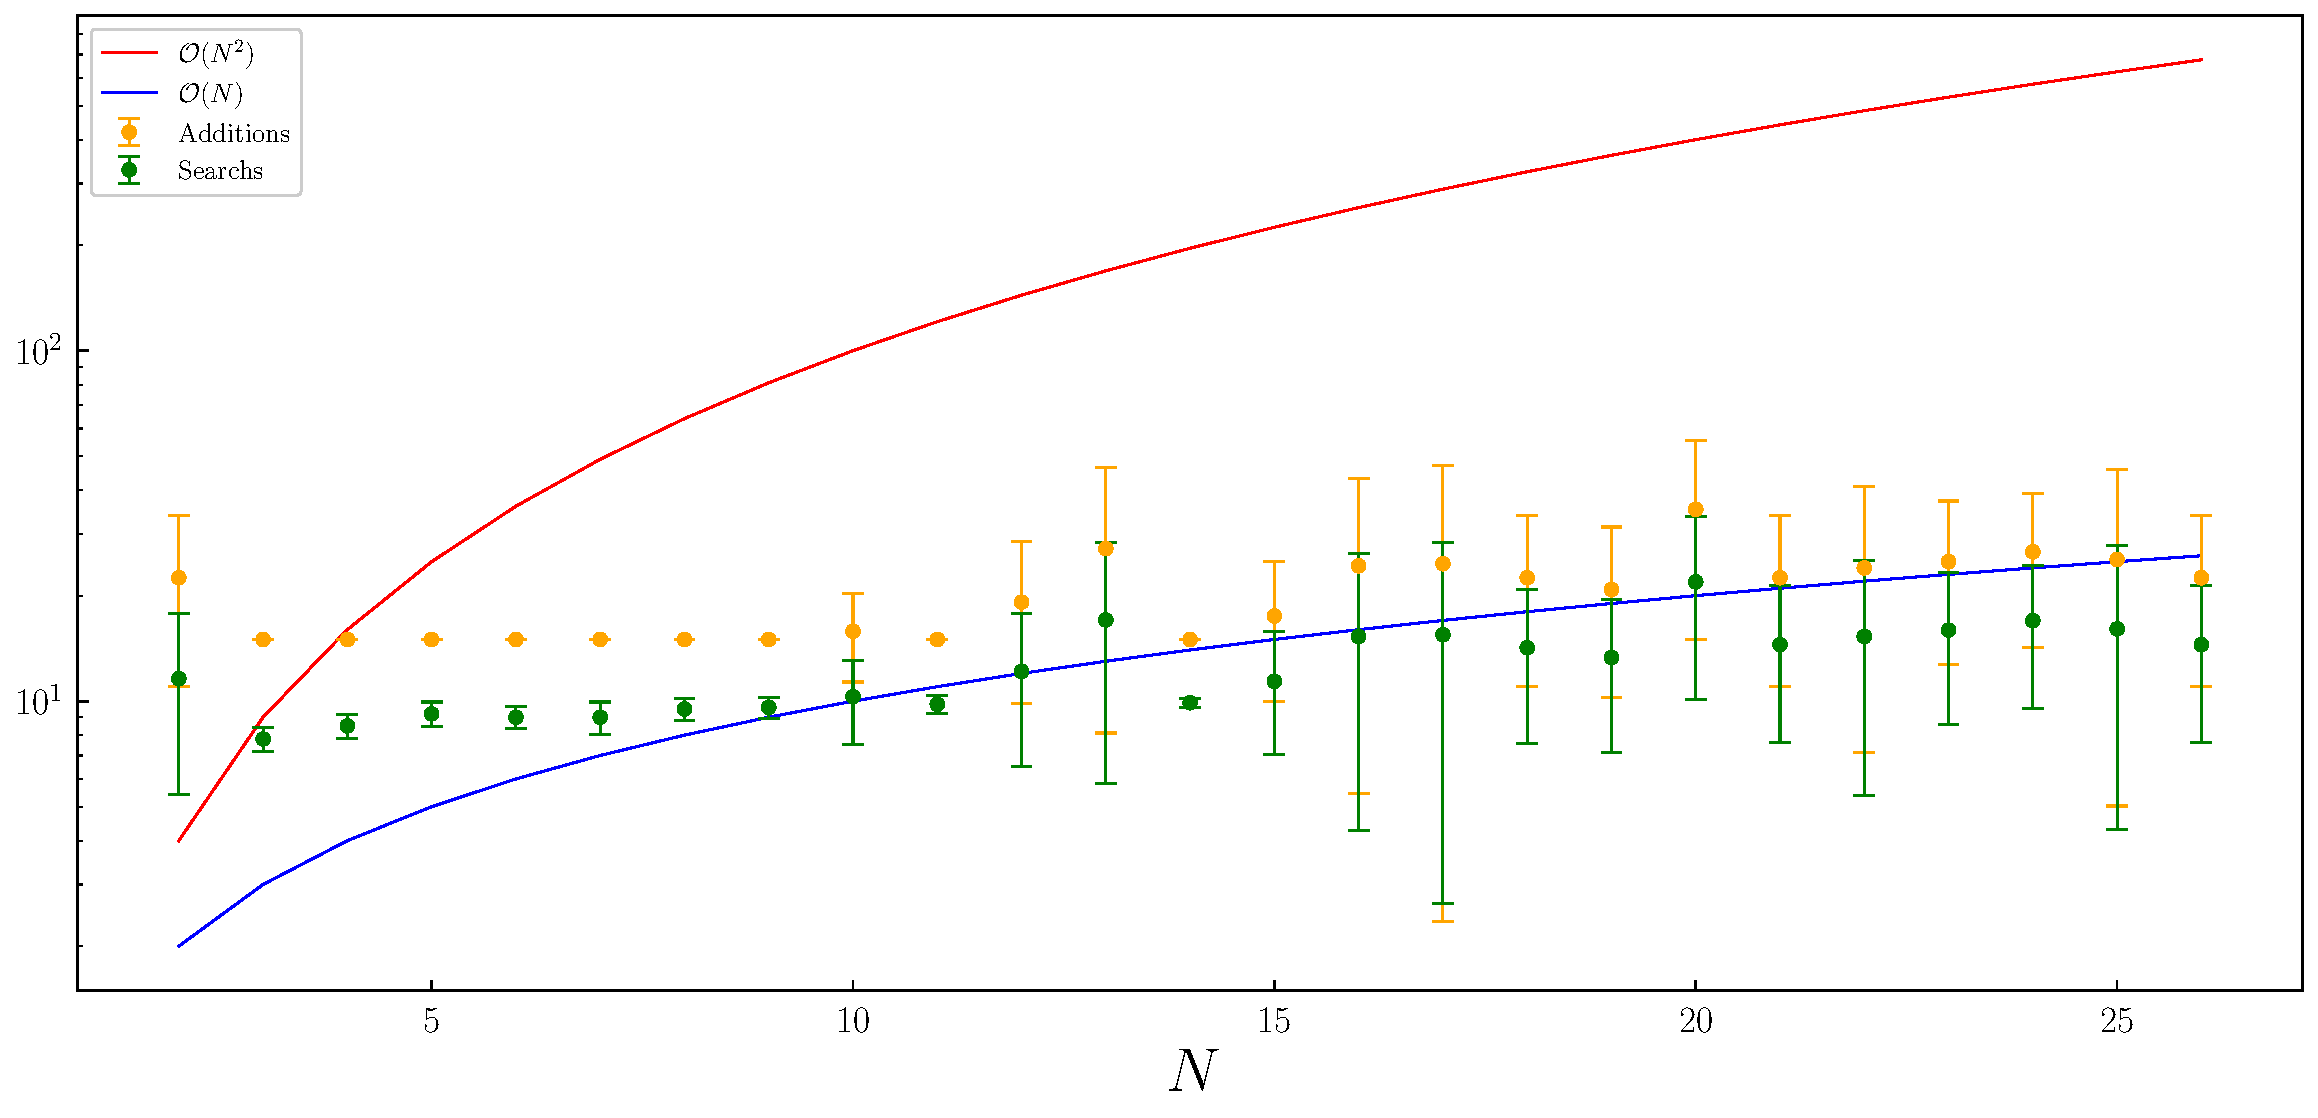
\includegraphics[width=0.8\textwidth]{../Results/Results.pdf}
        \caption{The plot illustrates the comparison of the number of additions (yellow) and searches (green) required to solve the problem for different sizes of prime number lists $N$. As the size $N$ of the problem increases, the proposed quantum circuit outperforms the classical approach, demonstrating its scalability and efficiency. The asymptotic complexity of the naive classical solution is $\mathcal{O}(N^2)$ (red), while the theoretical quantum asymptotic complexity is $\mathcal{O}(N)$ (blue).}
        \label{fig:Results}
    \end{figure}

    \section{Conclusion}

    In conclusion, this work has presented a quantum algorithm for verifying Goldbach's conjecture, a mathematical hypothesis that posits that any even integer greater than two can be expressed as the sum of two prime numbers. The proposed quantum circuit leverages quantum parallelism and the Grover's algorithm to efficiently search for pairs of prime numbers that add up to a given even integer.

    Through a comprehensive analysis, it has been shown that the quantum approach exhibits a favorable asymptotic complexity of $O(N)$ compared to the naive classical approach, which has an asymptotic complexity of $\mathcal{O}(N^2)$. This indicates that as the size of the problem grows, the quantum solution becomes significantly more efficient than its classical counterpart.

    Simulation results have confirmed the effectiveness of the proposed quantum circuit, solving the problem for various even integers and prime number lists. While the classical approach remains competitive for small-sized prime lists, the quantum solution shines as the problem size increases.

    Overall, this study demonstrates the potential of quantum computing to tackle complex mathematical problems efficiently and highlights the scalability and efficiency advantages of quantum algorithms in comparison to classical methods. The findings encourage further exploration of quantum computing's capabilities in addressing mathematical conjectures and computational challenges.


    \nocite{*}
    \bibliographystyle{unsrt}
    \bibliography{bibliography}

\end{document}
